% Made up for the tikra benchmark.
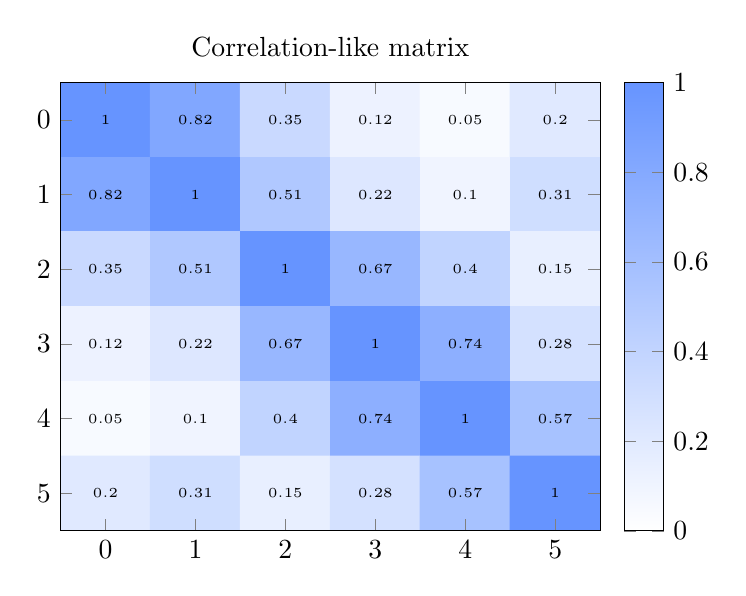
\begin{tikzpicture}
\begin{axis}[colormap={paleblue}{color=(white) color=(cyan!30!blue!60)}, colorbar, enlargelimits=false, axis on top, y dir=reverse,
    xtick={0,...,5}, ytick={0,...,5}, title={Correlation-like matrix}, point meta min=0,
    point meta max=1, nodes near coords={\pgfmathprintnumber[fixed, precision=2]{\pgfplotspointmeta}}, nodes near coords style={font=\tiny, anchor=center}]
  \addplot[matrix plot*, mesh/cols=6, point meta=explicit] table[meta=c] {
    x y c
    0 0 1.00
    1 0 0.82
    2 0 0.35
    3 0 0.12
    4 0 0.05
    5 0 0.20
    0 1 0.82
    1 1 1.00
    2 1 0.51
    3 1 0.22
    4 1 0.10
    5 1 0.31
    0 2 0.35
    1 2 0.51
    2 2 1.00
    3 2 0.67
    4 2 0.40
    5 2 0.15
    0 3 0.12
    1 3 0.22
    2 3 0.67
    3 3 1.00
    4 3 0.74
    5 3 0.28
    0 4 0.05
    1 4 0.10
    2 4 0.40
    3 4 0.74
    4 4 1.00
    5 4 0.57
    0 5 0.20
    1 5 0.31
    2 5 0.15
    3 5 0.28
    4 5 0.57
    5 5 1.00
  };
\end{axis}
\end{tikzpicture}
